\documentclass{standalone}
\def\pgfsysdriver{pgfsys-pdftex.def}%fading可能
\usepackage[usenames,dvipsnames,svgnames,x11names,table]{xcolor}
\usepackage{tikz}
\usetikzlibrary{arrows,positioning,automata,shadows,fit,shapes,patterns,fadings}
\usetikzlibrary{shadows}
\begin{document}
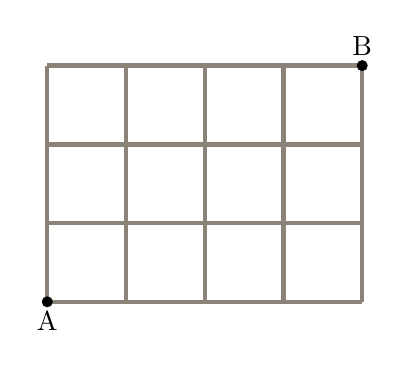
\begin{tikzpicture}
\draw [ultra thick,AntiqueWhite4] (0,0) grid (4,3);%(0,0)から(3,4)までの方眼
\fill(0,0) circle (2pt) node[below](0,0){A};
\fill(4,3) circle (2pt) node[above](4,3){B};
\end{tikzpicture}
\end{document}
